\documentclass{standalone}

\usepackage{tikz}
\usepackage{ifthen}
\usepackage[default]{gfsneohellenic}
\usepackage[LGR,T1]{fontenc} %% LGR encoding is needed for loading the package gfsneohellenic

\begin{document}

	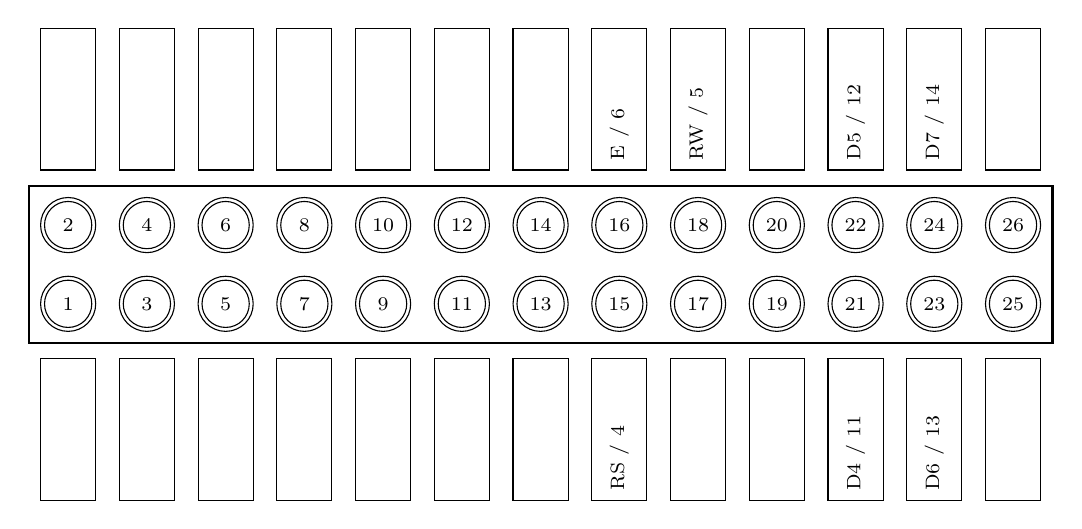
\begin{tikzpicture}

		% Frame
		\draw[thick] (0,0) rectangle (13,2);

		% Pins and rectangles
		\tikzstyle{every node}=[font=\scriptsize]
		\foreach \x [
			evaluate = \x as \toppin using int(\x*2),
			evaluate = \x as \bottompin using int(\x*2-1)
		] in {1,...,13} {
			\draw (\x-0.5,1.5) node {\toppin} circle (0.3) circle (0.35);
			\draw (\x-0.5,0.5) node {\bottompin} circle (0.3) circle (0.35);
			\draw (\x-0.85,2.2) rectangle (\x-0.15,4);
			\draw (\x-0.85,-0.2) rectangle (\x-0.15,-2);
		}

		% Labelling function
		\newcommand{\pinlabel}[2]{%
			\ifthenelse{\isodd{#1}}%
			{\node[anchor=west,rotate=90] at (#1/2, -2) {#2}}%
			{\node[anchor=west,rotate=90] at (#1/2-0.5, 2.2) {#2}}
		};

		% Labels
		\pinlabel{15}{RS / 4};
		\pinlabel{16}{E / 6};
		\pinlabel{18}{RW / 5};
		\pinlabel{21}{D4 / 11};
		\pinlabel{22}{D5 / 12};
		\pinlabel{23}{D6 / 13};
		\pinlabel{24}{D7 / 14};

	\end{tikzpicture}

\end{document}
